\documentclass{article}

\usepackage[paper=letterpaper,margin=2.5cm]{geometry} % Set Margins

%% Math and math fonts
\usepackage{amsmath, amsthm, amssymb, amsfonts}
\usepackage{bbm} % for \mathbbm{1}

% date
\usepackage[nodayofweek]{datetime}

% Color
\usepackage{color, xcolor}

% Misc
\usepackage{environ}  % \collect@body in asmmath
\usepackage{graphicx} % \includegraphics options
\usepackage{mdframed} % text boxes
\usepackage{indentfirst} % Indent first paragraph after section header
\usepackage{comment} % Comments
\usepackage{fancyhdr} % Headers and footers

% Tables
\usepackage{array}

% Sub-figures and figure placement
\usepackage{caption}
\usepackage{subcaption}
\usepackage{float} 

% Graphing
\usepackage{pgfplots}
\pgfplotsset{compat=1.17}
\usepackage{tikz}

% Title Placement
\usepackage{titling}
\setlength{\droptitle}{-6em}

%set indent to 
\setlength{\parindent}{0pt}

% Hyper refs
\usepackage{hyperref}
\hypersetup{
    colorlinks=true,
    linkcolor=blue,
    urlcolor  = blue,
    filecolor=magenta,      
    urlcolor=blue,
    citecolor = blue,
    anchorcolor = blue
}

% % Citation management
\usepackage{natbib}
\bibliographystyle{abbrvnat}
\setcitestyle{authordate,open={(},close={)}}

\pagestyle{fancy}

\usepackage[paper=letterpaper,margin=2.5cm]{geometry} % Set Margins

%% Math and math fonts
\usepackage{amsmath, amsthm, amssymb, amsfonts}
\usepackage{bbm} % for \mathbbm{1}

% date
\usepackage[nodayofweek]{datetime}

% Color
\usepackage{color, xcolor}

% Misc
\usepackage{environ}  % \collect@body in asmmath
\usepackage{graphicx} % \includegraphics options
\usepackage{mdframed} % text boxes
\usepackage{indentfirst} % Indent first paragraph after section header
\usepackage{comment} % Comments
\usepackage{fancyhdr} % Headers and footers

% Tables
\usepackage{array}

% Sub-figures and figure placement
\usepackage{caption}
% \usepackage{subcaption}
\usepackage{float} 

% Graphing
\usepackage{pgfplots}
\pgfplotsset{compat=1.17}
\usepackage{tikz}

% Title Placement
\usepackage{titling}
\setlength{\droptitle}{-6em}

%set indent to 
\setlength{\parindent}{0pt}

% Hyper refs
\usepackage{hyperref}
\hypersetup{
    colorlinks=true,
    linkcolor=blue,
    urlcolor  = blue,
    filecolor=magenta,      
    urlcolor=blue,
    citecolor = blue,
    anchorcolor = blue
}

% % Citation management
\usepackage{natbib}
\bibliographystyle{abbrvnat}
\setcitestyle{authordate,open={(},close={)}}

\newcolumntype{M}{>{$}c<{$}} % Define a new column type for math mode


% ----------------------------------------
% TITLE
% ----------------------------------------

\pagestyle{fancy}

\lhead{Creel}
\chead{Eigenvalues and eigenvectors}
\rhead{AMES}

\title{AMES Week 13 class notes -- Weds, Constrained Optimization}
\author{Andie Creel}

\begin{document}
\maketitle
\section{Introduction}
We learned how to find the maximums of a function \textit{when the function has a maximum}. For example, consider a population of bears and we want to know the population level where their population is growing the fastest \textit{i.e.} what's the population that leads to the maximum growth rate?\\

Let's work through this refresher example:
\begin{align}
    g = x(1 - x)
\end{align}
where $g$ is the growth rate and $x$ is the population level. \\

Find the $x$ that maximizes $g$. 

\begin{align}
    \frac{d g}{d x} = 1 - 2x = 0\\
   \implies x^* = \frac{1}{2}
\end{align}

But what about if the function just keeps increasing, and it's your budget that constrains how much you can maximize? 

\begin{figure}[htp]
    \centering
    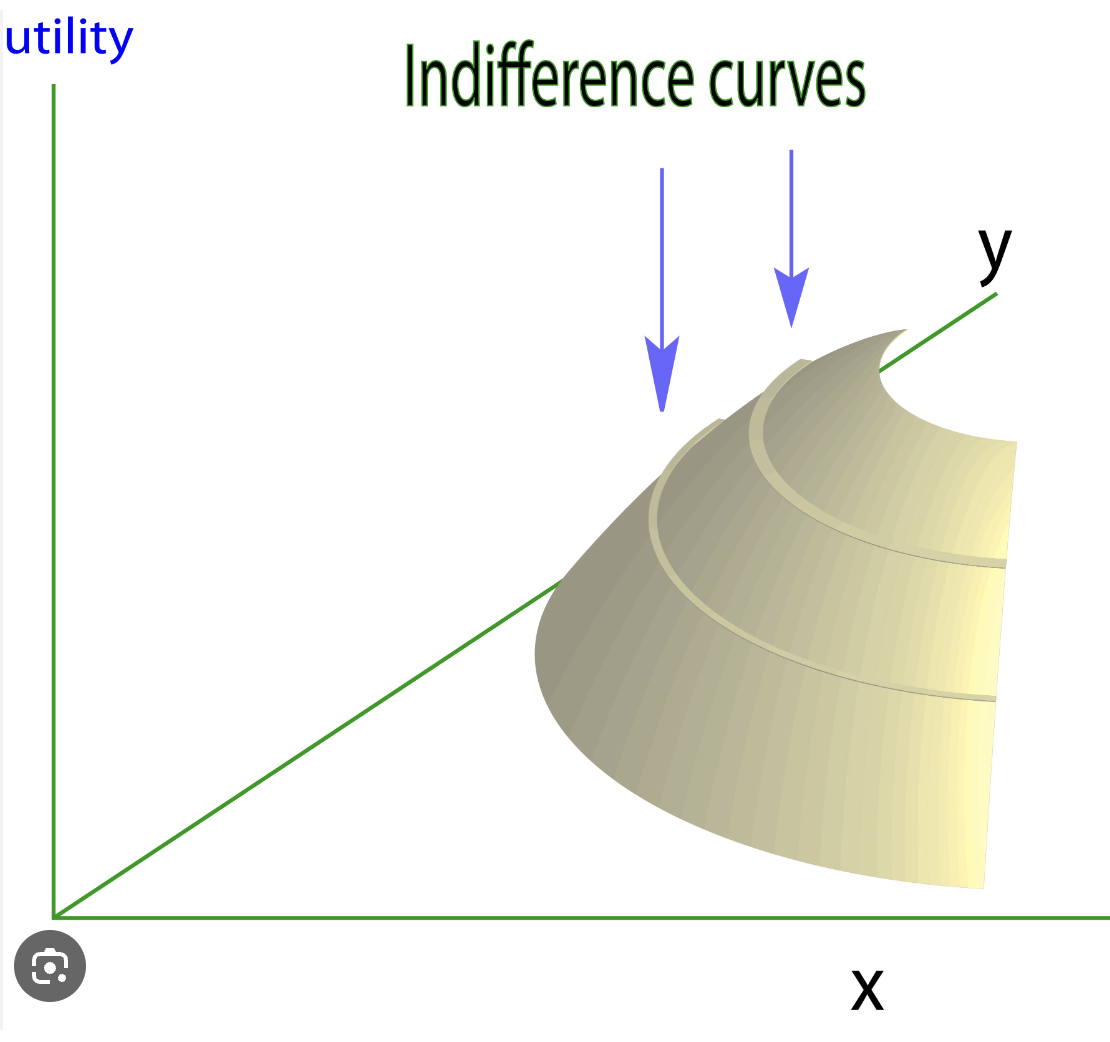
\includegraphics[width=0.5\linewidth]{Screen Shot 2023-12-01 at 1.17.20 PM.png}
    \caption{Constantly increasing function (no obvi maximum)}
    \label{fig:enter-label}
\end{figure}
This is a function where $U$ just keeps increasing as the $(x,y)$ point gets further away from the origin. So if we want to maximize $U$ but choosing $x$ and $y$ we'd choose infinite of each. \\

\begin{figure}[htp]
    \centering
    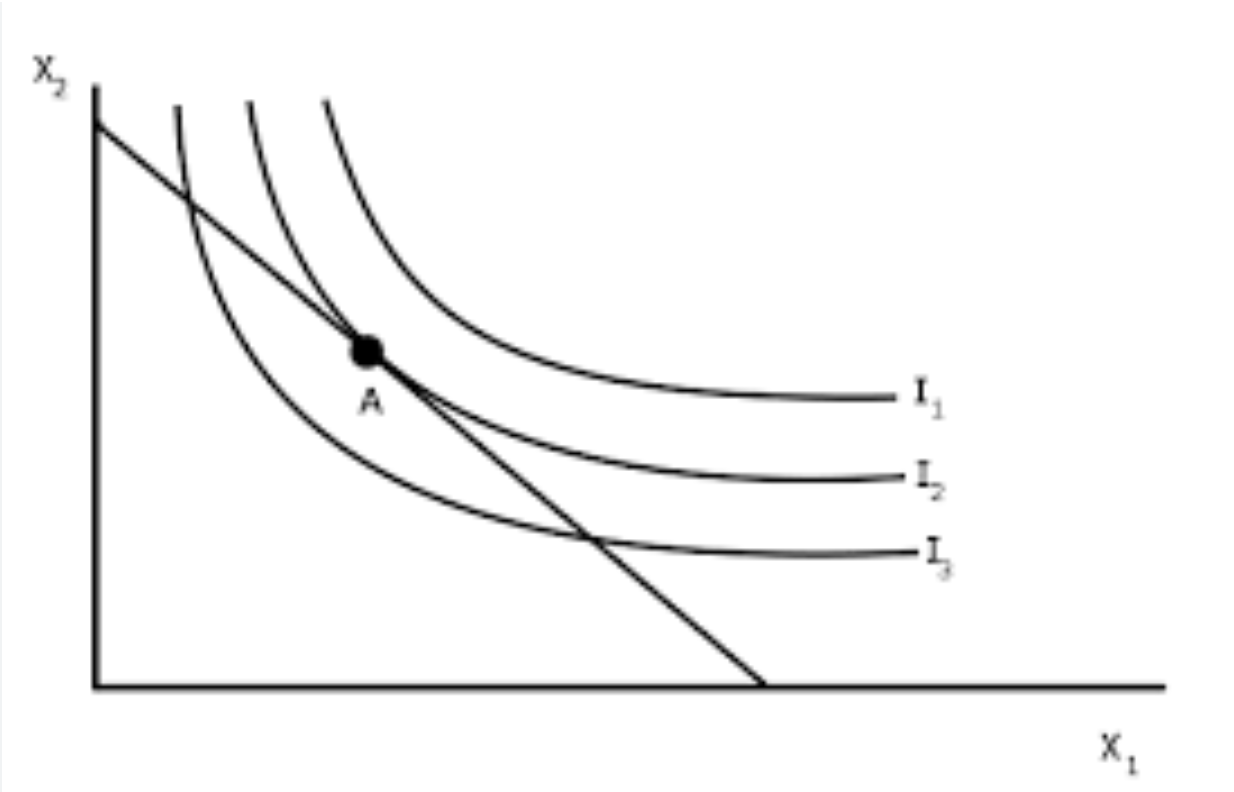
\includegraphics[width=0.5\linewidth]{Screen Shot 2023-12-01 at 1.18.52 PM.png}
    \caption{Birds eye view of same figure, straight line is the budget}
    \label{fig:enter-label}
\end{figure}

But let's say you can't afford infinite $x$ and infinite $y$. You have a constraint on the amount of $x$ and $y$ you can have. This is what we call \textbf{constrained optimizations} and we use a \textbf{Lagrangian} to solve these problems. 

\section{Lagrangians}
I think the most common example of constrained optimization people in this room will see is utility maximization with a budget constraint. \\

We use Lagrangians to solve for the optimal quantity of goods to consume in order to maximize a utility function, subject to a budget constraint.\\

A note on the word consume: traditionally, economists only thought people increased their utility by "consuming goods". In this class, we know people gain utility from flowers,  park visits, or grizzly bear sightings. I still use the word consume for these non-consumptive goods for conciseness. 


\subsection{Utility function}
A utility function measures the welfare we get from consuming goods (this use can be consumptive or non-consumptive). Utility functions can take different functional forms, a common one is Cobb-Douglas 
$$U(x,y) = x^\alpha y^{1-\alpha}.$$

In this case, the individual only consumes two goods, good $x$ and good $y$.\\

\textbf{Our goal is to maximize utility subject to a constraint. }

\subsection{Constraint}
If we could, we'd consume infinite $x$ and infinite $y$ because utility increases with the consumption of goods. However, we typically have a "budget" of how much $x$ and how much $y$ we can buy. Let $B$ denote this budget, $p_x$ denote the price of $x$ and $p_y$ denote the price of y. The money we spend on $x$ and $y$ needs to be less than our budget,
$$p_x x + p_y y \leq B.$$
Because we want consume as much $x$ and $y$ as possible, this will become an equality rather than a less than or equal sign, 
$$p_x x + p_y y = B.$$
Note that we can rewrite our constraint as 
\begin{align}
    0 = B - p_x x + p_y y
    \label{constraint}
\end{align}

where we manipulate the constraint to \textit{equal zero}. 

\subsection{Constrained optimization of utility}
Our goal is to maximize utility subject to our constraint. We will write down a \textbf{Lagrangian}, which will become the function we want to maximize. 

\begin{align}
    L &= U(x, y) + 0 \\
    &= U(x, y) + \lambda (B - p_x x + p_y y) \label{lagrange}
\end{align}

Our Lagrangian is our utility function \textit{plus zero}, because $\lambda$ multiplied by equation \ref{constraint} is zero. So maximizing the Lagrangian is the same as maximizing our utility, but we're incorporating our constraint. \\

The term $\lambda$ is referred to as the \textit{marginal utility of money}. This is because $\frac{d L}{d B} = \lambda$. This interpretation is important for natural capital accounting, but is not important for this class. \\

We want to solve for the optimal level of consumption of goods $x^*$ and $y^*$ to maximize $U(x,y)$. \\

We take the derivatives and set them equal to zero to find the maximum. We call this \textbf{first order conditions (FOC)}, which are also known as the \textbf{optimality conditions}\\

FOCs:
\begin{align}
    \frac{\partial L}{\partial x} =... = 0 \label{foc_x}\\
    \frac{\partial L}{\partial y} =... = 0 \label{foc_y}\\
    \frac{\partial L}{\partial \lambda} =... = 0 \label{constraint_foc}
\end{align}

The FOCs gives us three equations (\ref{foc_x} - \ref{constraint_foc}) and three unknowns ($x$, $y$, $\lambda$). We can solve for the optimal $x^*$ and $y^*$. We can also solve for $\lambda$, which is the marginal utility of money in the Lagrangian case.

\section{Example}
Let's consider an explicit example. 

\begin{align*}
    U(x, y) = x^\frac{1}{2} y^\frac{1}{2}\\
    B = 10\\
    p_x = 1\\
    p_y = 2
\end{align*}
Our budget constraint will be 
\begin{align*}
    10 = x + 2 y\\
    10 - x - 2y = 0 
\end{align*}

Our Lagrangian will be 
\begin{align*}
    L = x^\frac{1}{2} y^\frac{1}{2} + \lambda( 10 - x - 2y)
\end{align*}

FOCs:
\begin{align}
    \frac{\partial L}{\partial y} = \frac{1}{2} x^\frac{1}{2} y^{-\frac{1}{2}}-\lambda 2 = 0 \label{dy}\\
    \frac{\partial L}{\partial x} = \frac{1}{2} x^{-\frac{1}{2}} y^{\frac{1}{2}}-\lambda  = 0 \label{dx}\\
    \frac{\partial L}{\partial \lambda} = 10 - x - 2y = 0 \label{const}
\end{align}
We now have 3 equations and 3 unknowns $x, y, \lambda$. We're not going to solve for $\lambda$ today, but once you have $x$ and $y$ you can.\\


Solve \ref{dy} and \ref{dx} for $\lambda$ and set these equations equal to one another to get: 
\begin{align*}
    \frac{\frac{1}{2} x^\frac{1}{2} y^{-\frac{1}{2}}}{2} = \frac{1}{2} x^{-\frac{1}{2}} y^{\frac{1}{2}} \\
    \frac{1}{2} x^\frac{1}{2} y^{-\frac{1}{2}} = x^{-\frac{1}{2}} y^{\frac{1}{2}}\\
    \frac{1}{2} x = y 
\end{align*}

we can plug $\frac{1}{2} x = y $ back into \ref{const}
\begin{align*}
    10 = x + 2 \frac{1}{2} x\\
    x^* = 5 
\end{align*}

and we can plug this value of $x^*$ into $\frac{1}{2} x = y $ to get 
\begin{align*}
    y = \frac{1}{2}x\\
    y^* = 2.5
\end{align*}

so the value of $(x,y)$ that maximized $U(x,y)$ subject to our budget constraint is $(5, 2.5)$. 

\end{document}
